%#!platex ./report.tex

%
% Rerative -> Relative
%
\section{Passive$B$N7k2L(B}
   \subsection{$B@h9T8&5f<jK!(B\cite{torben2009systematic}$B$H$NHf3S(B}
     $BK\8&5f<jK!$H@h9T8&5f$GMQ$$$i$l$F$$$?8DBNI>2A;XI8$H$NHf3S$r0J2<$N(B
     $B?^(B\ref{Tsuishi_Relative1}, $B?^(B\ref{Tsuishi_Relative2}$B$K<($9(B. 
     $B?^Cf$N(BTorben et al.$B$O@h9T8&5f<jK!$rMQ$$$?7k2L$G$"$j(B, Relative$B$OK\8&5f$rMQ$$$?7k2L$G$"$k(B.

%subfigure $B$rF~$l$k$H$-$K2~9T$9$k$H!"<B:]$NJ8>O$G$b2~9T$,H?1G$5$l!"2#$KJB$P$J$/$J$k$k$N$GCm0U(B
     \begin{figure}[H]
       \begin{subfigure}{0.5\columnwidth}
         \centering
         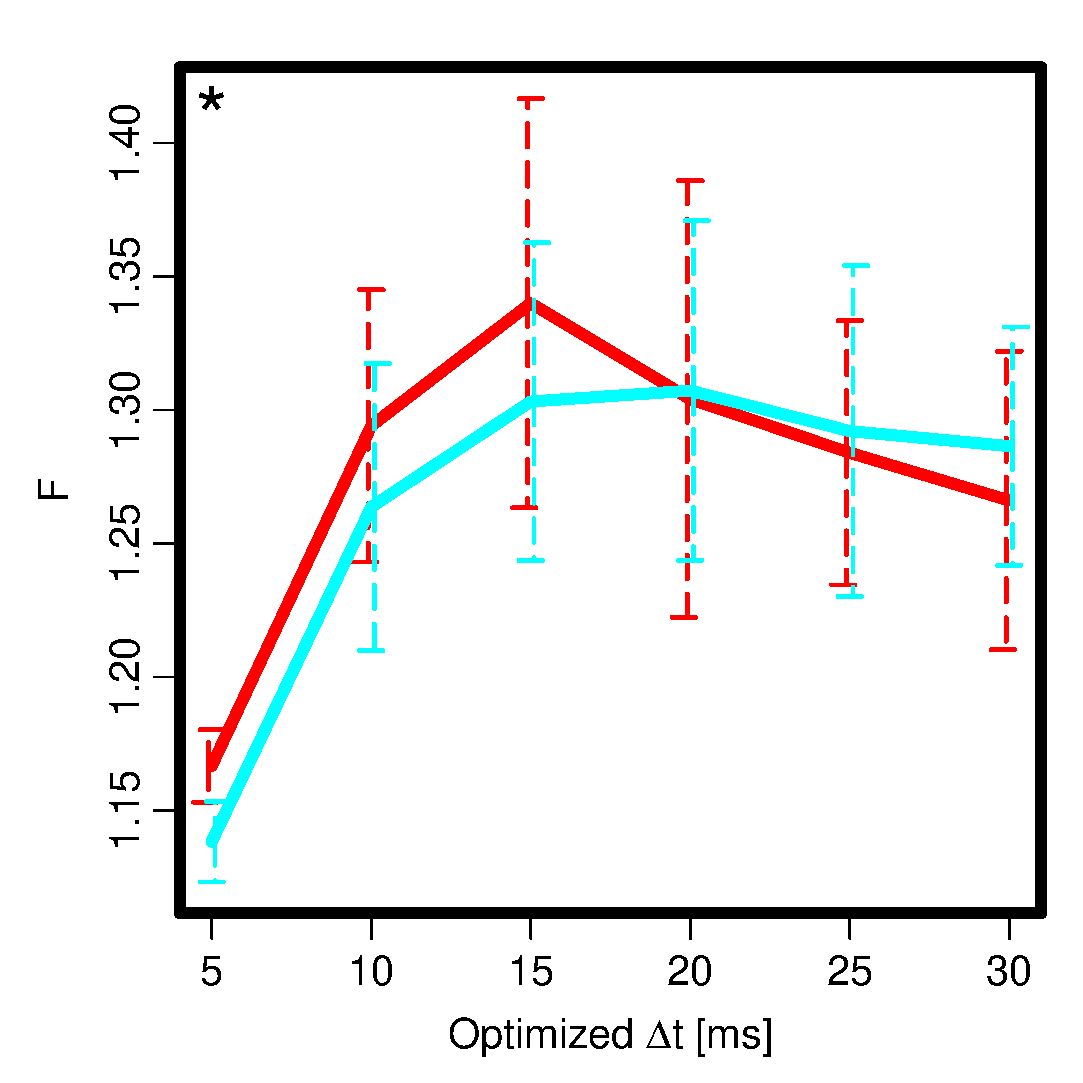
\includegraphics[width=0.8\columnwidth]{./Images_Result/Tsuishi_Rerative_F.eps} 
         \caption{F}
         \label{Tsuishi_Relative_F}
       \end{subfigure}
       \begin{subfigure}{0.5\columnwidth}
         \centering
         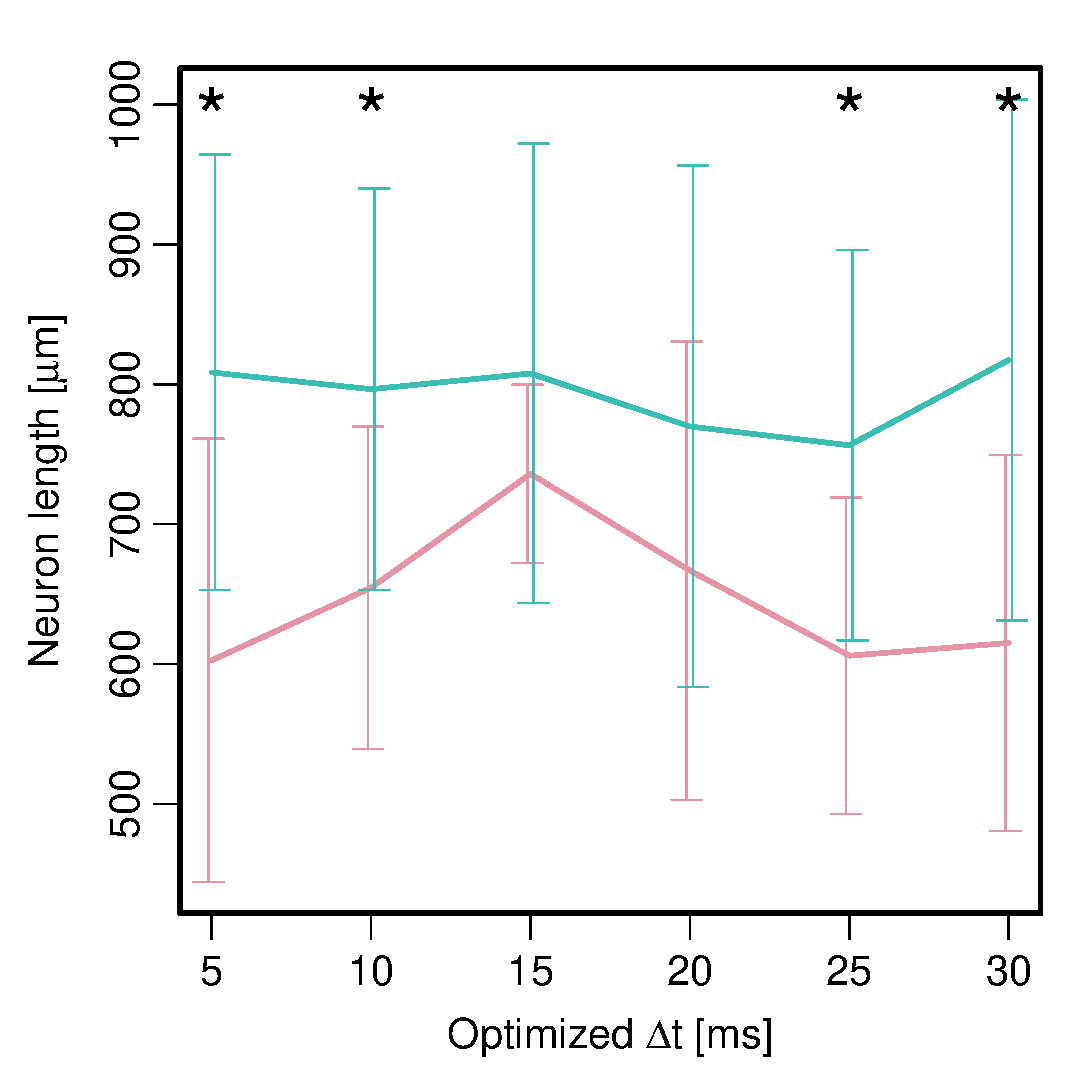
\includegraphics[width=0.8\columnwidth]{./Images_Result/Tsuishi_Rerative_TREE_length.eps} 
         \caption{$BD9$5(B}
         \label{Tsuishi_Relative_length}
       \end{subfigure}

       \begin{subfigure}{0.5\columnwidth}
         \centering
         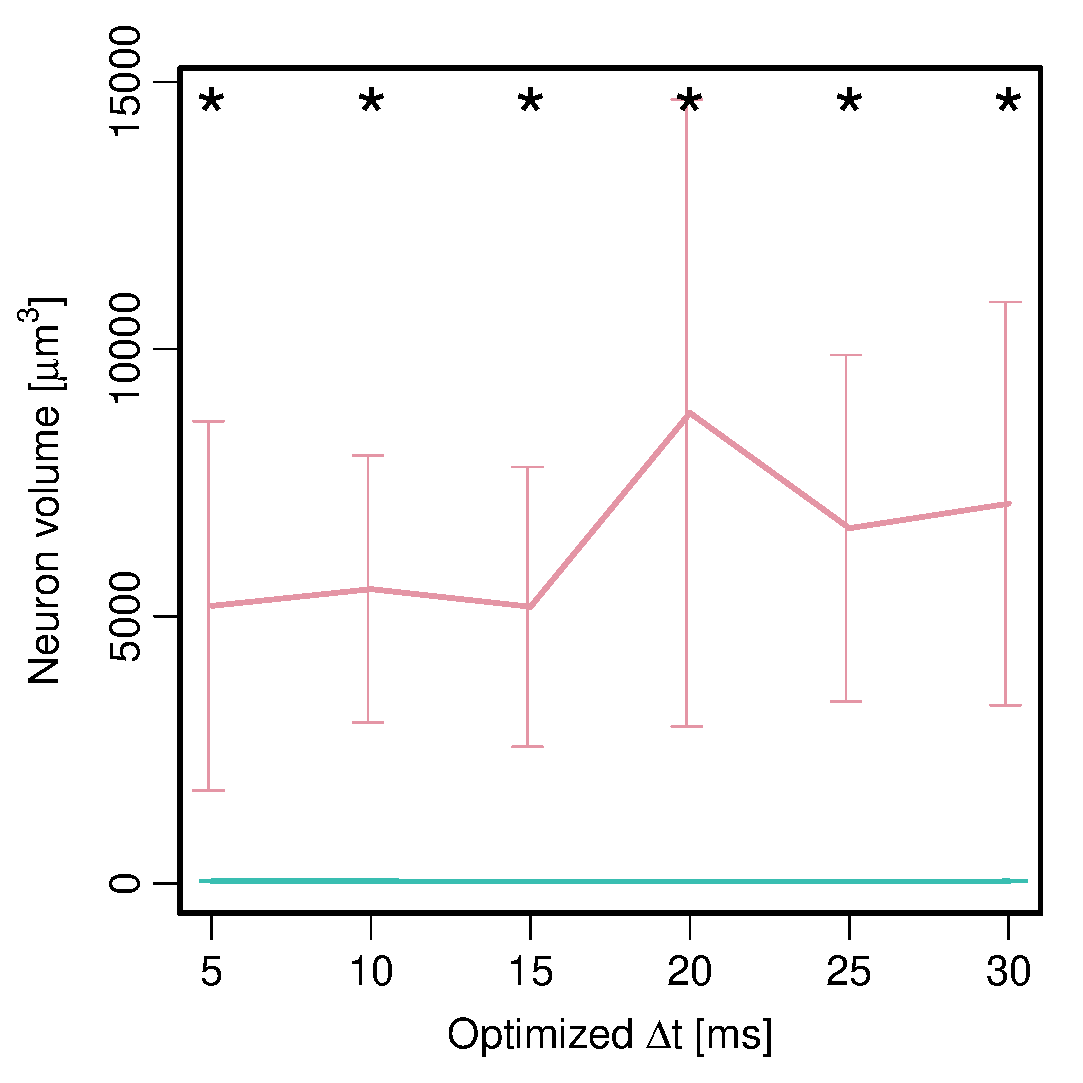
\includegraphics[width=0.8\columnwidth]{./Images_Result/Tsuishi_Rerative_TREE_volume.eps} 
         \caption{$BBN@Q(B}
         \label{Tsuishi_Relative_volume}
       \end{subfigure}
       \begin{subfigure}{0.5\columnwidth}
         \centering
         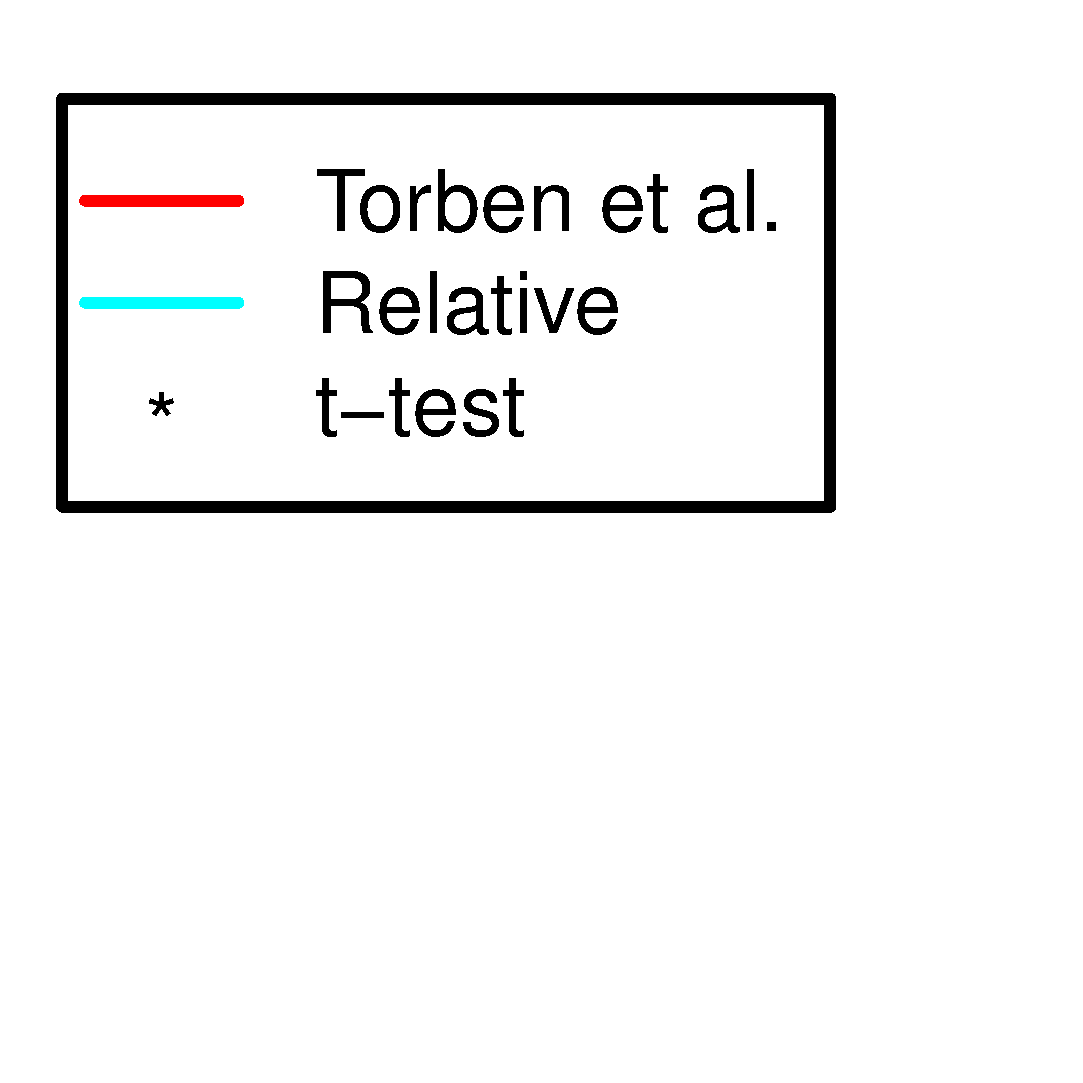
\includegraphics[width=0.8\columnwidth]{./Images_Result/Tsuishi_Rerative_legend.eps} 
       \end{subfigure}

       \caption{$B@h9T8&5f<jK!$H$NHf3S(B1}
       \label{Tsuishi_Relative1}
     \end{figure}

     \begin{figure}[H]
       \begin{subfigure}{0.5\columnwidth}
         \centering
         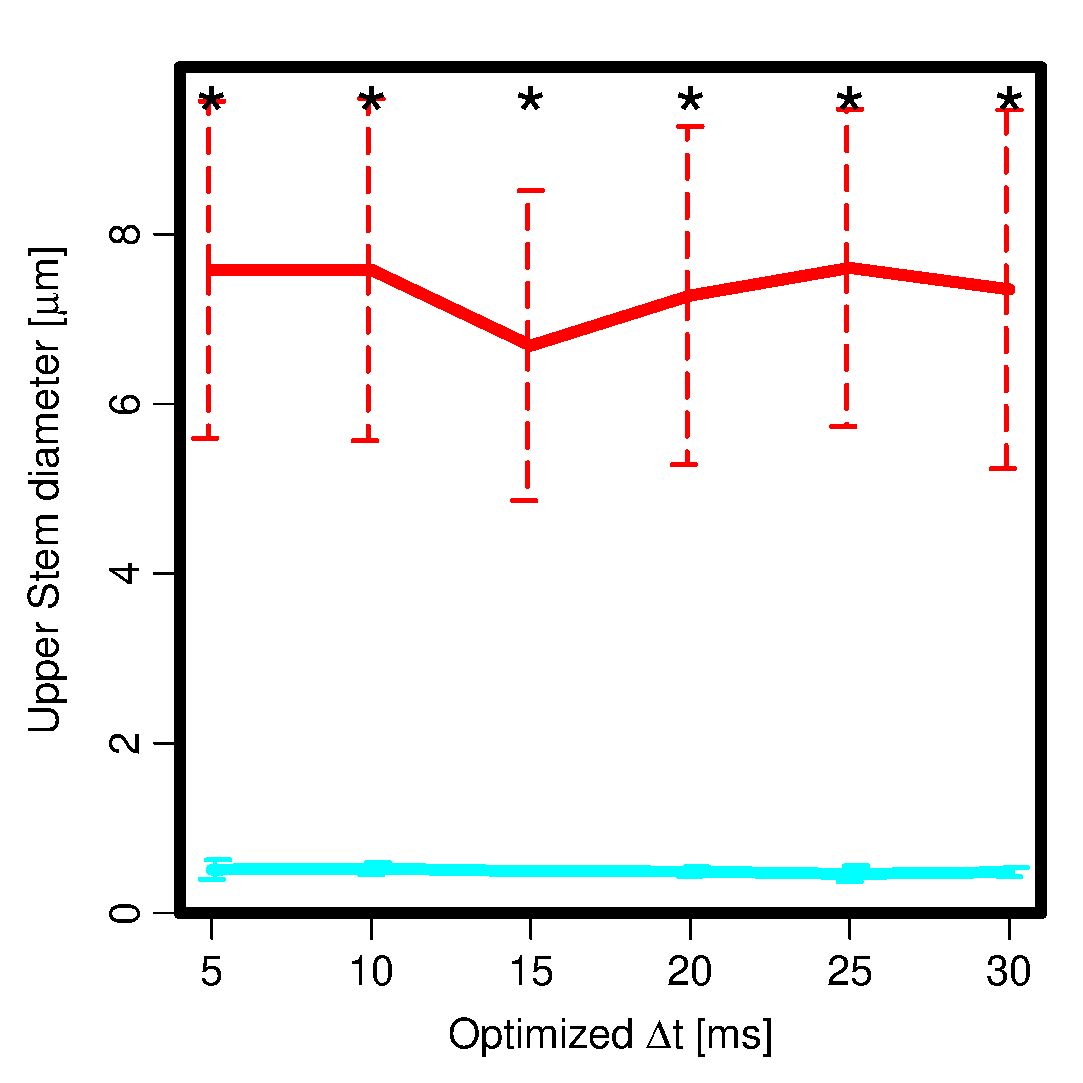
\includegraphics[width=0.8\columnwidth]{./Images_Result/Tsuishi_Rerative_Upper_Diam.eps} 
         \caption{Upper Dendrite$B$ND>7B(B}
         \label{Tsuishi_Relative_Upper_Diam}
       \end{subfigure}
       \begin{subfigure}{0.5\columnwidth}
         \centering
         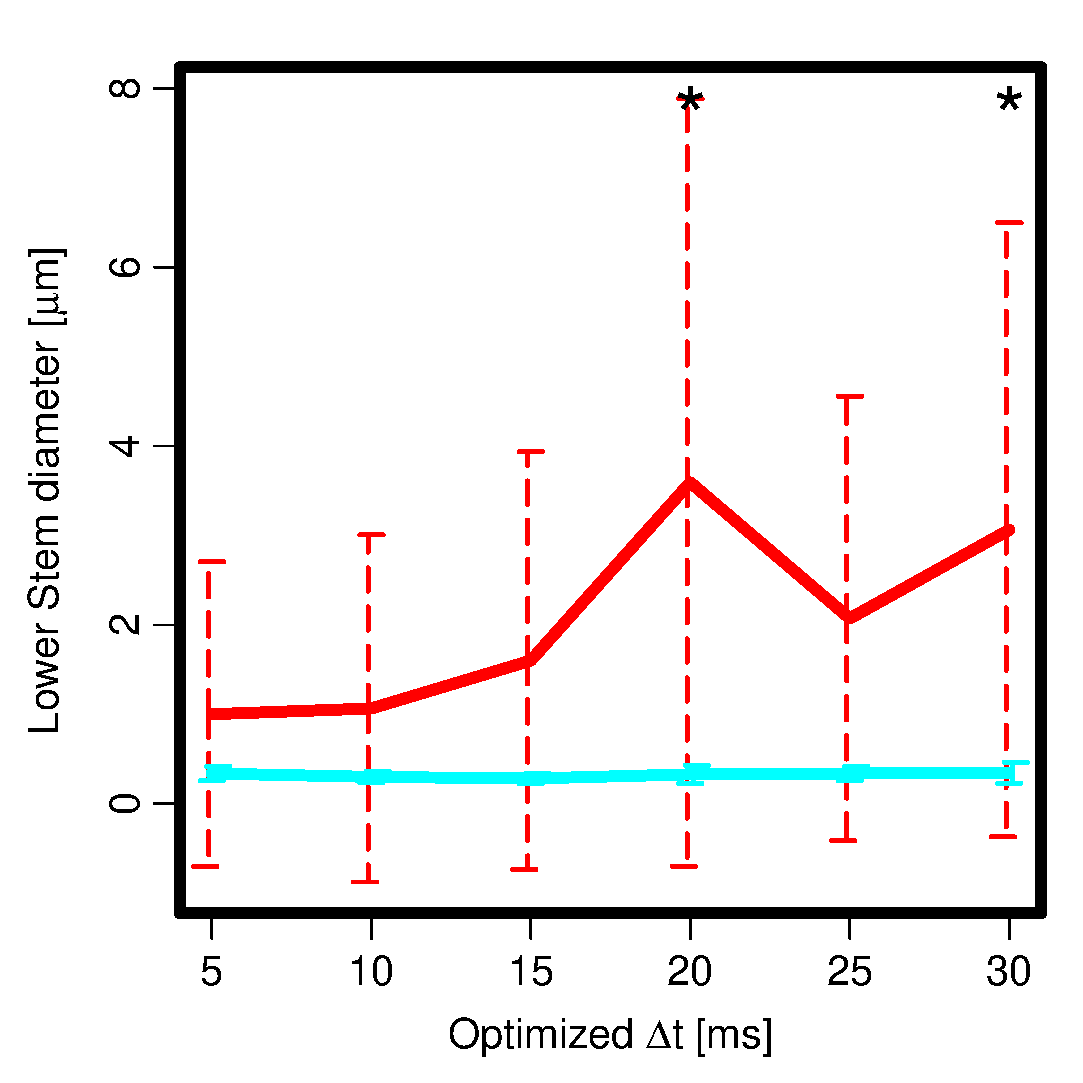
\includegraphics[width=0.8\columnwidth]{./Images_Result/Tsuishi_Rerative_Lower_Diam.eps} 
         \caption{Lower Dendrite$B$ND>7B(B}
         \label{Tsuishi_Relative_Lower_Diam}
       \end{subfigure}

       \caption{$B@h9T8&5f<jK!$H$NHf3S(B2}
       \label{Tsuishi_Relative2}
     \end{figure}

     $B3F(B${\Delta}t$$B$K$*$$$F?^Cf>eIt$N@10u(B(${\star}$)$B$O(B, $B%&%'%k%A$N(Bt$B8!Dj(B(${\alpha} = 0.05$)
     $B$rMQ$$$F(B
     $B@h9T8&5f<jK!(B(Torben et al)$B$HK\8&5f<jK!(B(Relative)$B$NJ?6QCM$rHf3S$7$?:]$K(B
     $BM-0Y:9$,$_$i$l$?$3$H$r<($9(B. 
     $B?^(B\ref{Tsuishi_Relative_F}$B$H?^(B\ref{Tsuishi_Relative_volume}$B$r$_$k$H(B
     2$B$D$N<jK!$N4V$G5!G=@-(B$F$$B$K$O$"$^$j:9$O8+$i$l$J$$$,(B
     $BBN@Q$OL@$i$+$K>.$5$/$J$C$F$$$k$3$H$,$o$+$k(B. $B?^(B\ref{Tsuishi_Relative_Upper_Diam}$B$H(B
     \ref{Tsuishi_Relative_Lower_Diam}$B$O(B, $B$=$N860x$,<y>uFM5/$ND>7B$,>.$5$/$J$C$?$3$H(B
     $B$K$"$k$H<($7$F$$$k(B. \\
     $B?^(B\ref{Relative_Neuron_result}$B$OK\8&5f<jK!$K$h$C$FF@$i$l$??@7P:YK&(B
     $B$NBN@Q$K$D$$$F(B, $B?^(B\ref{Relative_Dend_result}$B$O(B2$B$D$N<y>uFM5/$4$H$NB@$5(B
     ($B?^(B\ref{Relative_Diam})$B$H7A@.$5$l$?%7%J%W%9$N8D?t(B($B?^(B\ref{Relative_N_Syn})$B$r<($9(B.
     
     \begin{figure}[H]
       \centering
       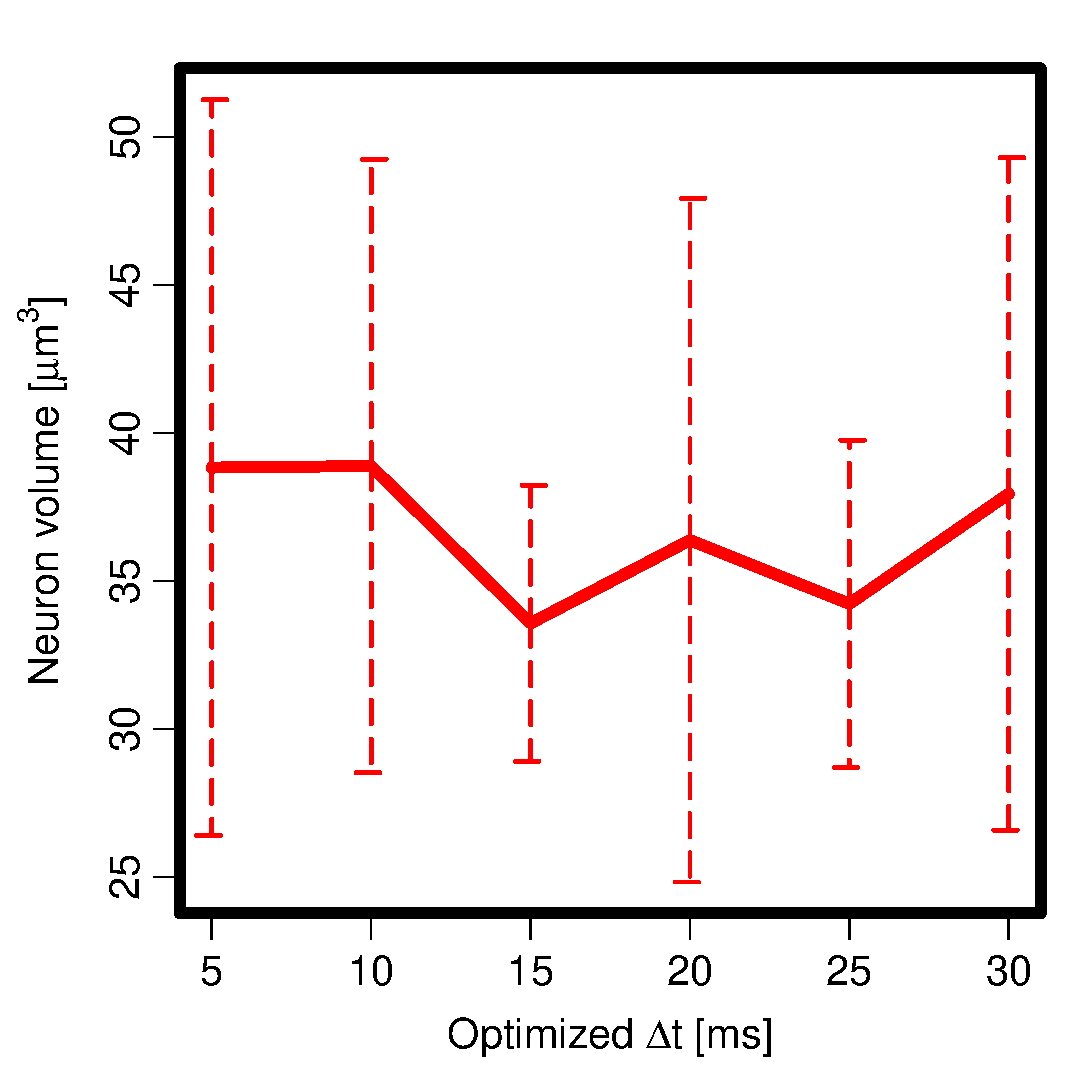
\includegraphics[width=0.4\columnwidth]{./Images_Result/passive_one_TREE_volume.eps}
       \caption{$BK\8&5f<jK!$GF@$i$l$??@7P:YK&$NBN@Q(B}
       \label{Relative_Neuron_result}
     \end{figure}

     \begin{figure}[H]
       \begin{subfigure}{0.5\columnwidth}
         \centering
         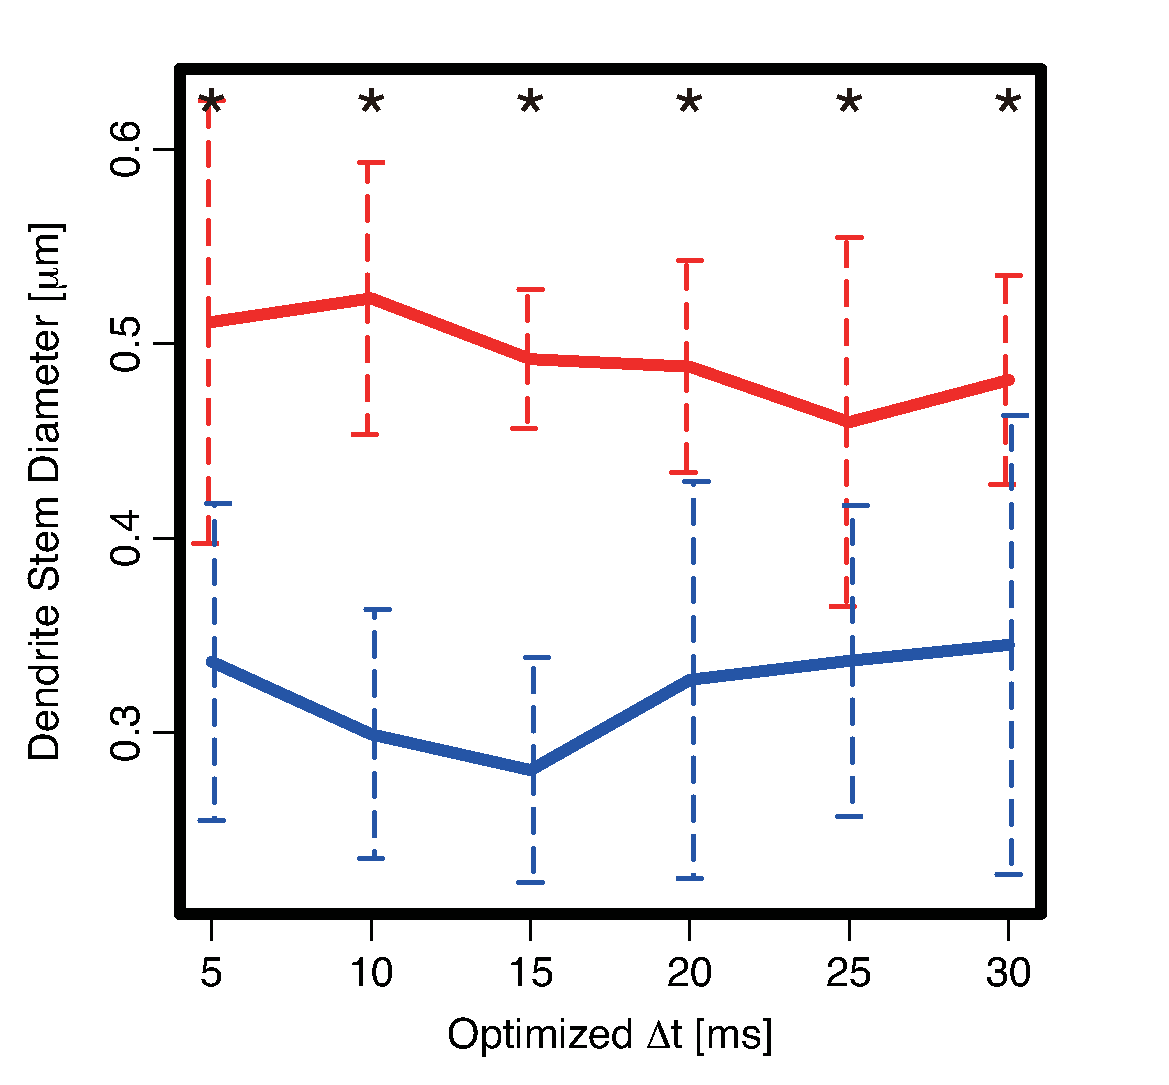
\includegraphics[width=0.8\columnwidth]{./Images_Result/passive_one_Dends_diam.eps}
         \caption{$B<y>uFM5/$ND>7B(B}
         \label{Relative_Diam}
       \end{subfigure}
       \begin{subfigure}{0.5\columnwidth}
         \centering
         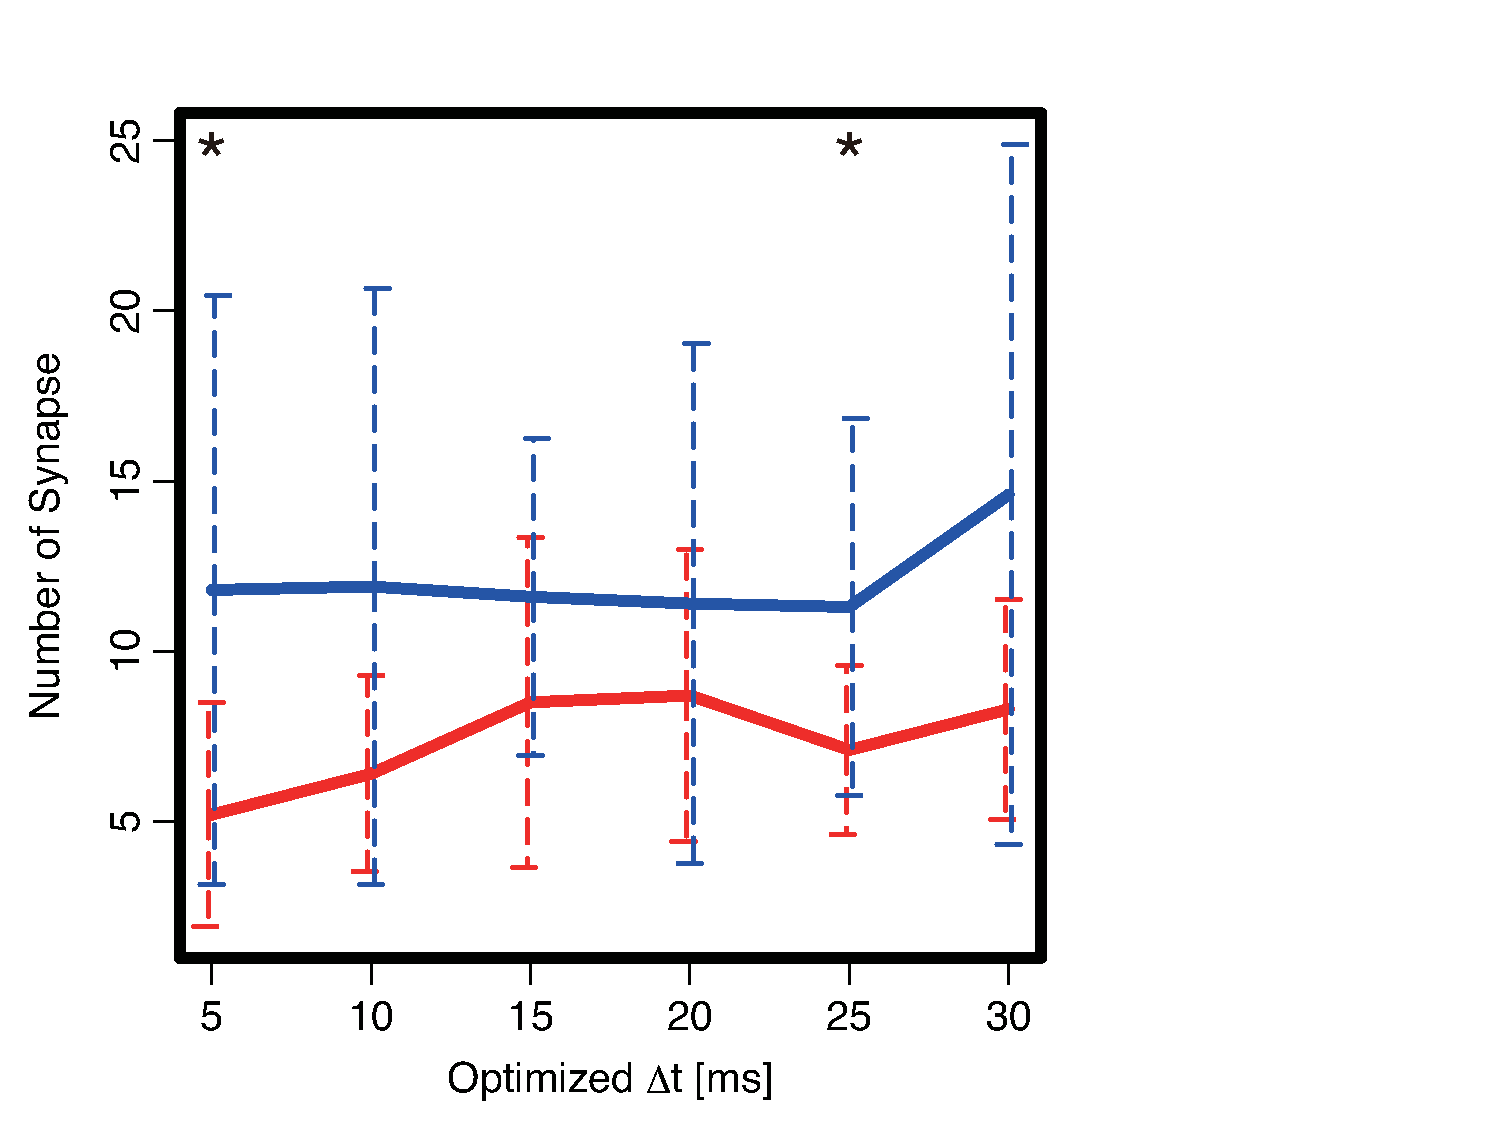
\includegraphics[width=1.05\columnwidth]{./Images_Result/passive_one_N_Dends_Syn.eps}
         \caption{Red $B%7%J%W%9(B, Blue $B%7%J%W%9$N8D?t(B}
         \label{Relative_N_Syn}
       \end{subfigure}
       \begin{subfigure}{\columnwidth}
         \centering
         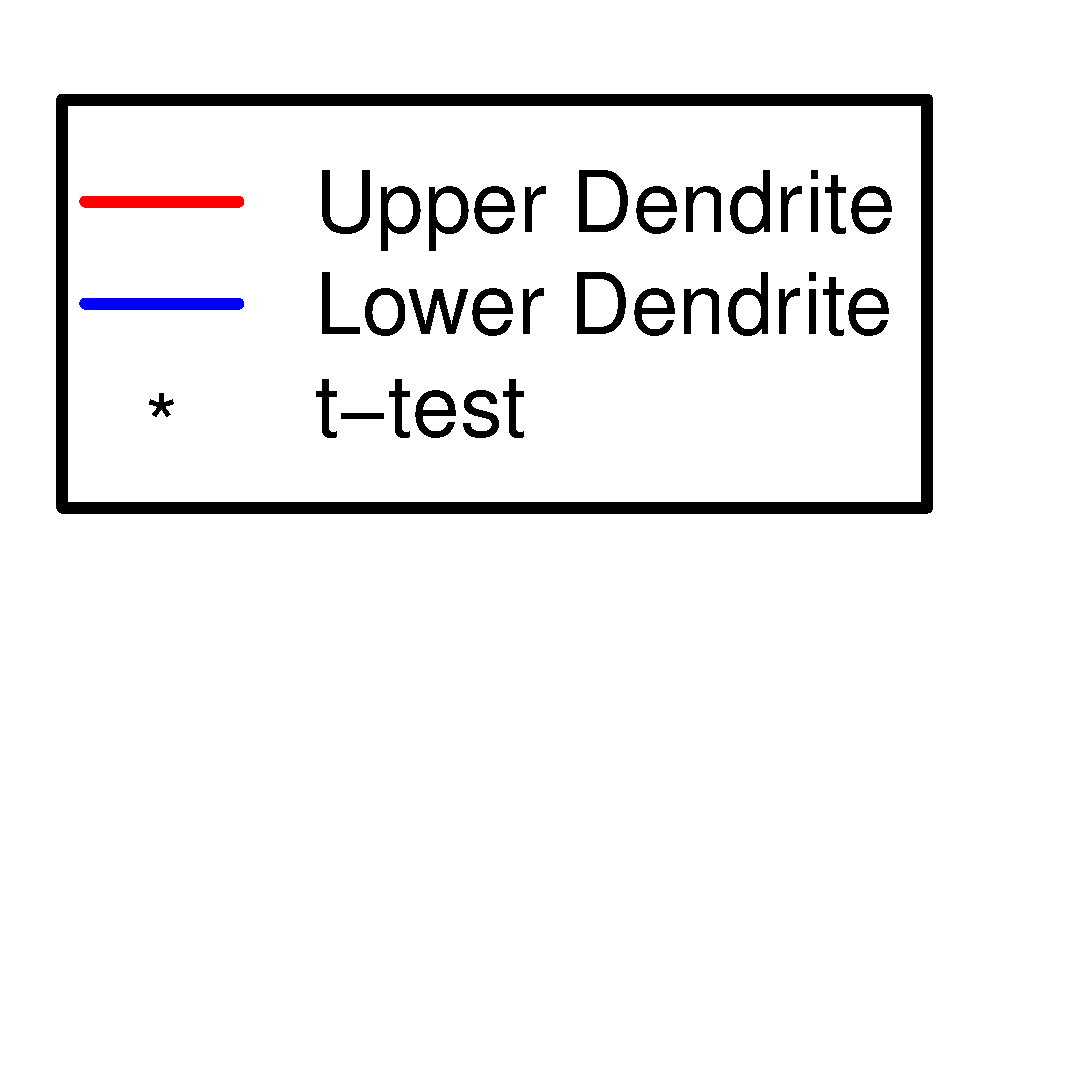
\includegraphics[width=0.3\columnwidth]{./Images_Result/passive_one_legend.eps}
       \end{subfigure}

       \vspace{-2cm}
       \caption{$BK\8&5f<jK!$GF@$i$l$?<y>uFM5/$N7ABV(B}
       \label{Relative_Dend_result}
     \end{figure}
     $B?^(B\ref{Relative_Diam}$B$G$_$i$l$k$h$&$K(BUpper Dendrite$B$ND>7B$O$9$Y$F$N(B${\Delta}t$$B$K$*$$$F(B
     $BL@$i$+$K(BLower Dendrite$B$h$j$bB@$$(B. $B$^$??^(B\ref{Relative_N_Syn}$B$K<($5$l$k$h$&$K(BBlue
     $B%7%J%W%9$N8D?t$,(BRed$B%7%J%W%9$N$*$h$=(B2$BG\DxEY$G$"$k(B. $B$3$N(B2$B$D$N7k2L$O@h9T8&5f$G$b(B
     $B<($5$l$F$$$k(B. \\     
     ${\Delta}t = 15$[ms]$B$K$*$$$F@h9T8&5f$N<jK!(B, $BK\8&5f$N<jK!$G@8@.$5$l$??@7P:YK&$NNc(B
     $B$r?^(B\ref{passive_morphos}$B$K<($9(B.

     \begin{figure}[H]
       \begin{subfigure}{0.5\columnwidth}
         \centering
         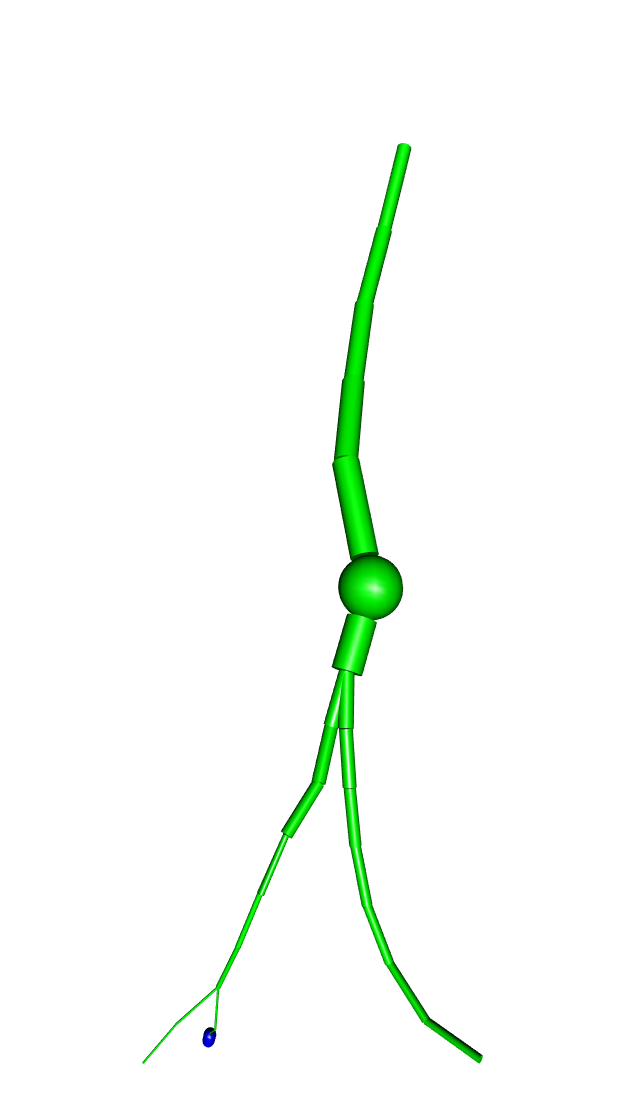
\includegraphics[width=0.4\columnwidth]{./Images_Result/alfa_sample.png} 
         \caption{$B@h9T8&5f<jK!(B}
         \label{Tsuishi_sampel}
       \end{subfigure}
       \begin{subfigure}{0.5\columnwidth}
         \centering
         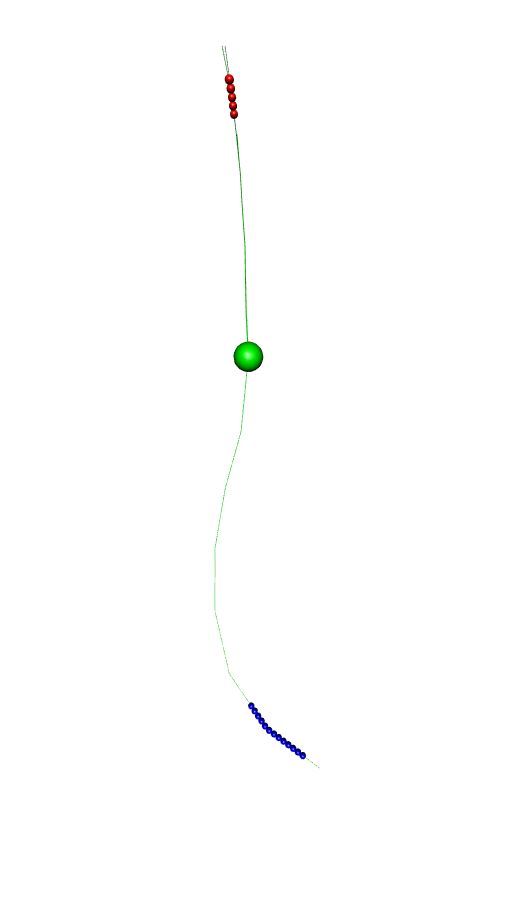
\includegraphics[width=0.3\columnwidth]{./Images_Result/rerative_sample.png}
         \caption{$BK\8&5f<jK!(B}
         \label{Relative_sampel}
       \end{subfigure}
       \caption{Passive$B$J?@7P:YK&$N7ABVNc(B}
       \label{passive_morphos}
     \end{figure}

     %% $B0J2<$N?^(B\ref{passive_syn}$B$OK\8&5f$N<jK!$G:n@.$7$??@7P:YK&$N(B, $B<y>uFM5/>e$N%7%J%W%97A@.0LCV(B
     %% $B$r<($7$F$$$k(B. $B?^Cf$N2#<4$O<y>uFM5/>e$N0LCV$rI=$7(B, 0[$\mu$m]$B$O:YK&BN$N0LCV$rI=$9(B.
     %% $B?^$G$O%7%J%W%9$rI=$94]0u$,=E$J$j@~$N$h$&$K$J$C$F$$$k$,(B, $B$3$l$O%7%J%W%9$,8_$$$K(B
     %% $B6a$$0LCV$KJ,I[$7$F$$$k$?$a$G$"$k(B. $B?^Cf$N<P@~$NItJ,$O%7%J%W%F%#%C%/%>!<%s$rI=$7$F$$$k(B. 
     %% %
     %% % $B%7%J%W%90LCV!"D9$5$N%0%i%U$O$b$&>/$72C9)$7$F$+$i=P$7$?J}$,$$$$(B
     %% %
     %% % $B%7%J%W%9$N?'$,0c$&(B!

     %% \begin{figure}[H]
     %%   \hspace*{-2cm}
     %%   \begin{subfigure}{0.62\columnwidth}
     %%     \centering
     %%     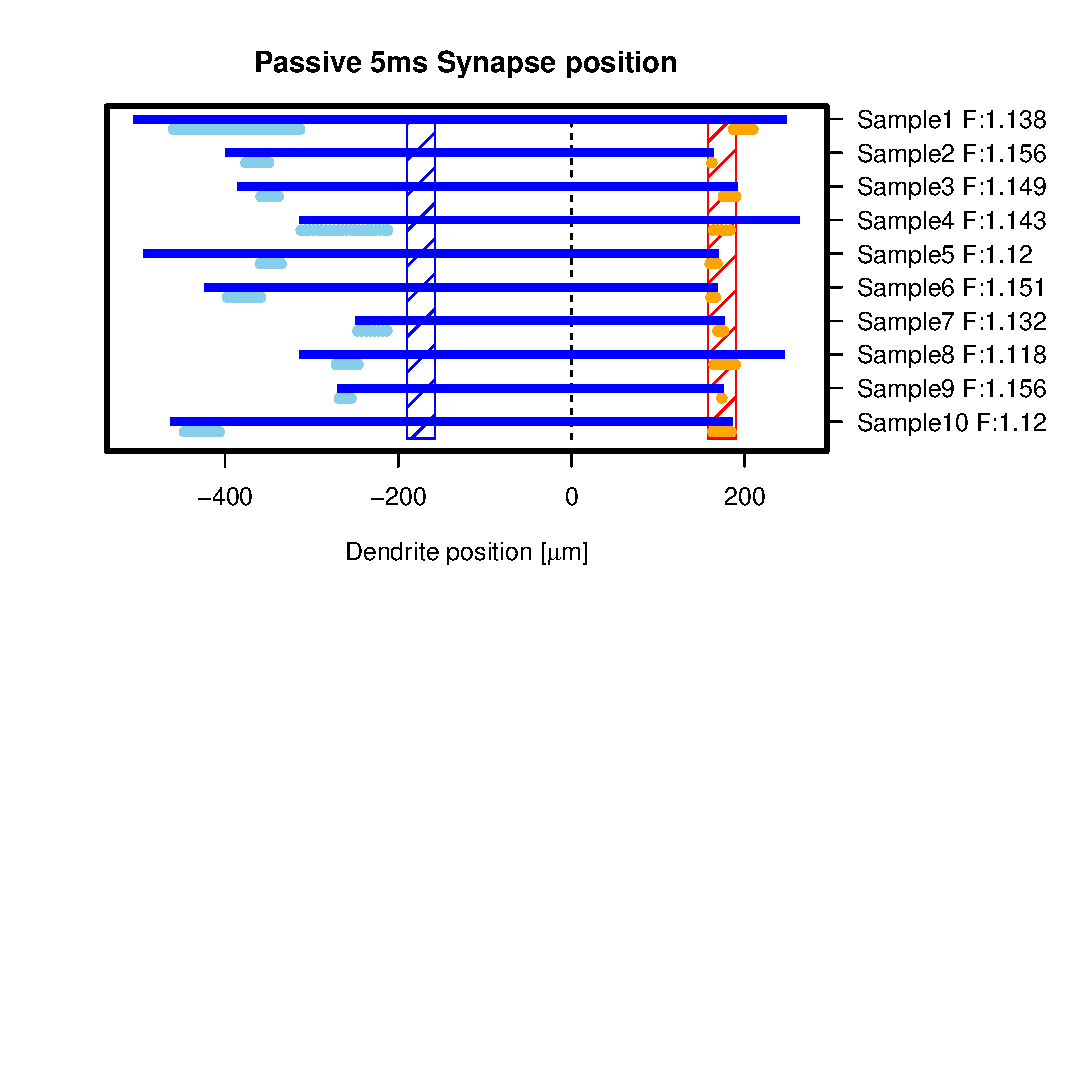
\includegraphics[width=\columnwidth]{./Images_Result/passive_Rerative_75_0_passive_syn_position_dt5.eps}
     %%     \vspace{-5cm}
     %%     \caption{${\Delta}t = 5$}
     %%     \label{passive_syn_dt=5}
     %%   \end{subfigure}
     %%   \begin{subfigure}{0.62\columnwidth}
     %%     \centering
     %%     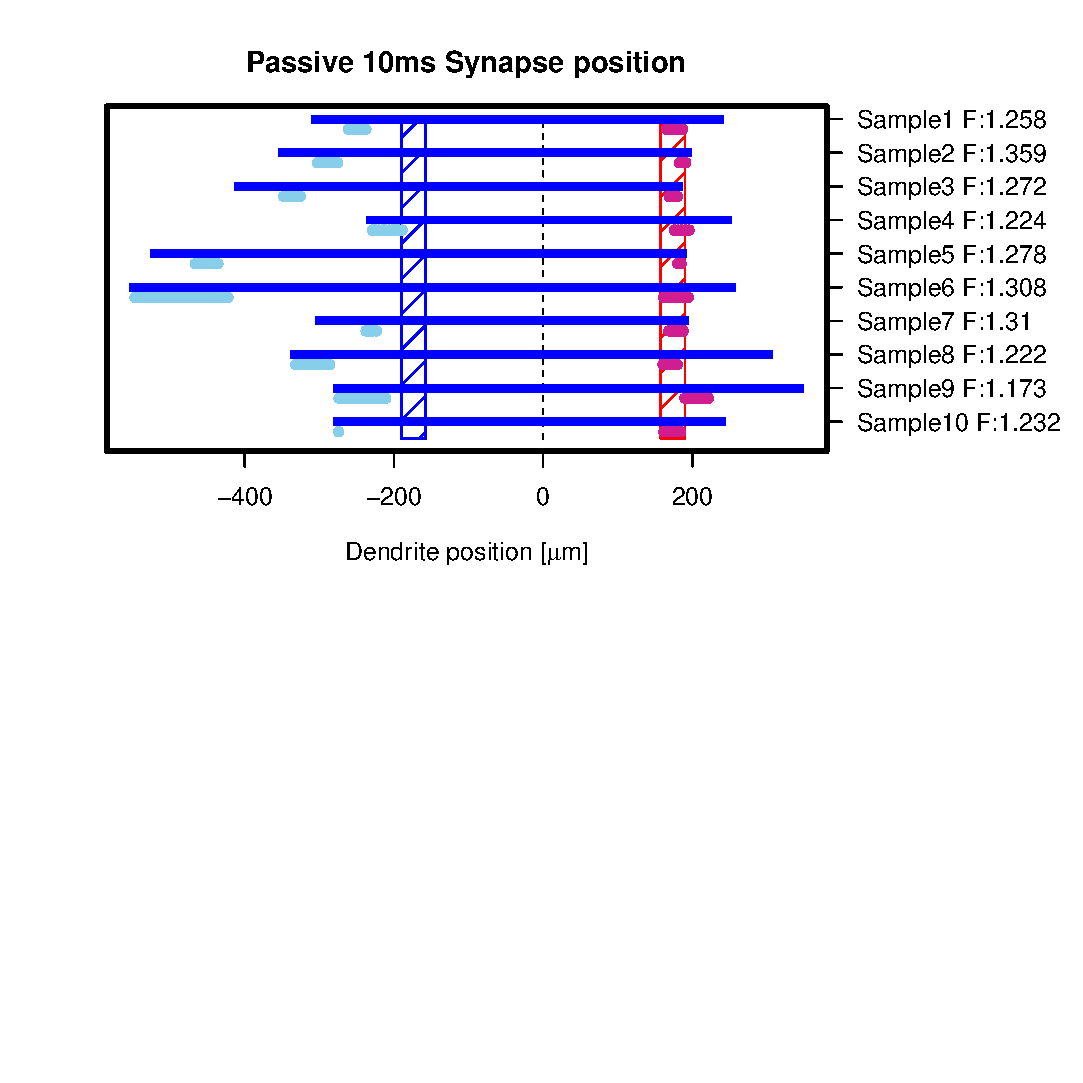
\includegraphics[width=\columnwidth]{./Images_Result/passive_Rerative_75_0_passive_syn_position_dt10.eps}
     %%     \vspace{-5cm}
     %%     \caption{${\Delta}t = 10$}
     %%     \label{passive_syn_dt=10}
     %%   \end{subfigure}

     %%   \hspace*{-2cm}
     %%   \begin{subfigure}{0.62\columnwidth}
     %%     \centering
     %%     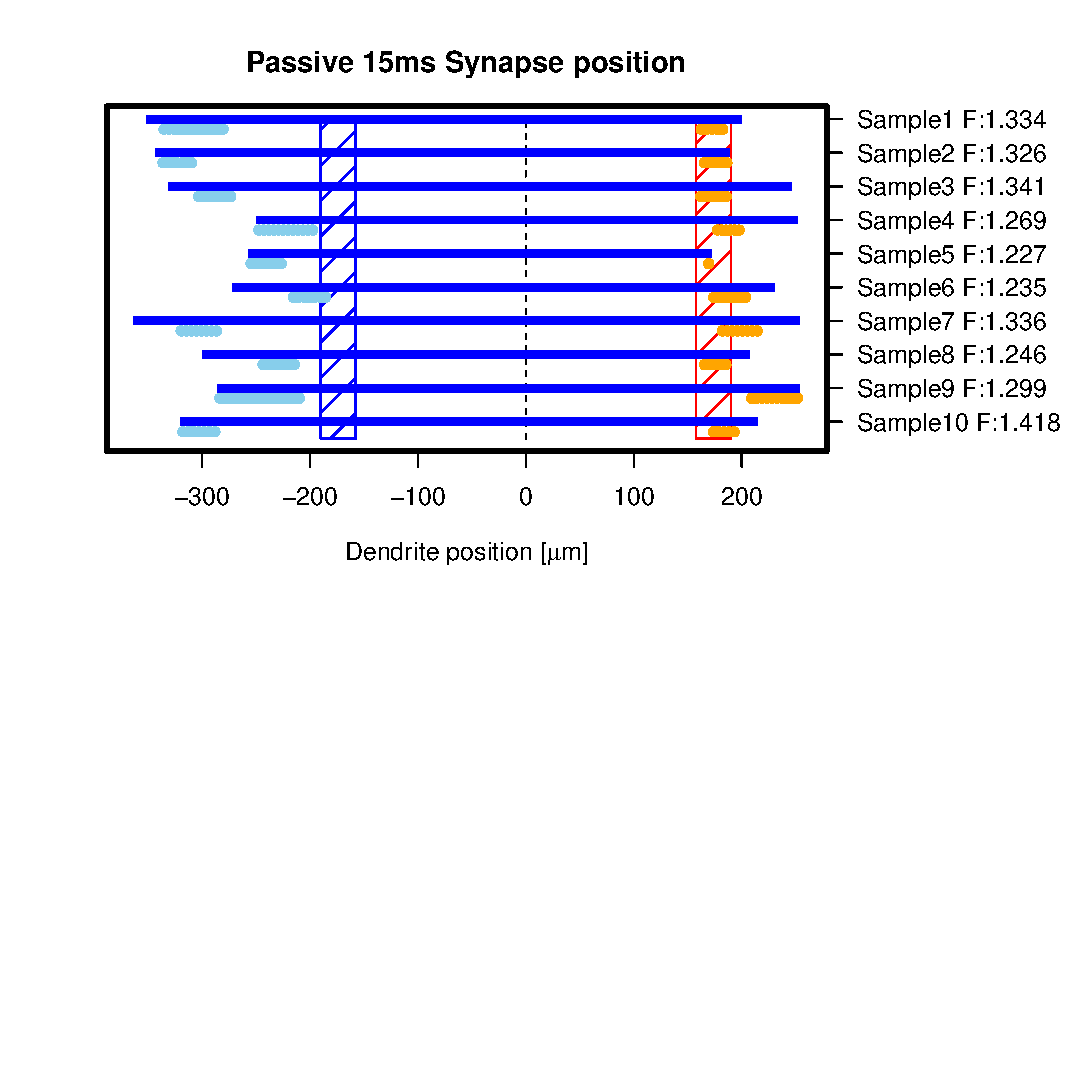
\includegraphics[width=\columnwidth]{./Images_Result/passive_Rerative_75_0_passive_syn_position_dt15.eps}
     %%     \vspace{-5cm}
     %%     \caption{${\Delta}t = 15$}
     %%     \label{passive_syn_dt=15}
     %%   \end{subfigure}
     %%   \begin{subfigure}{0.62\columnwidth}
     %%     \centering
     %%     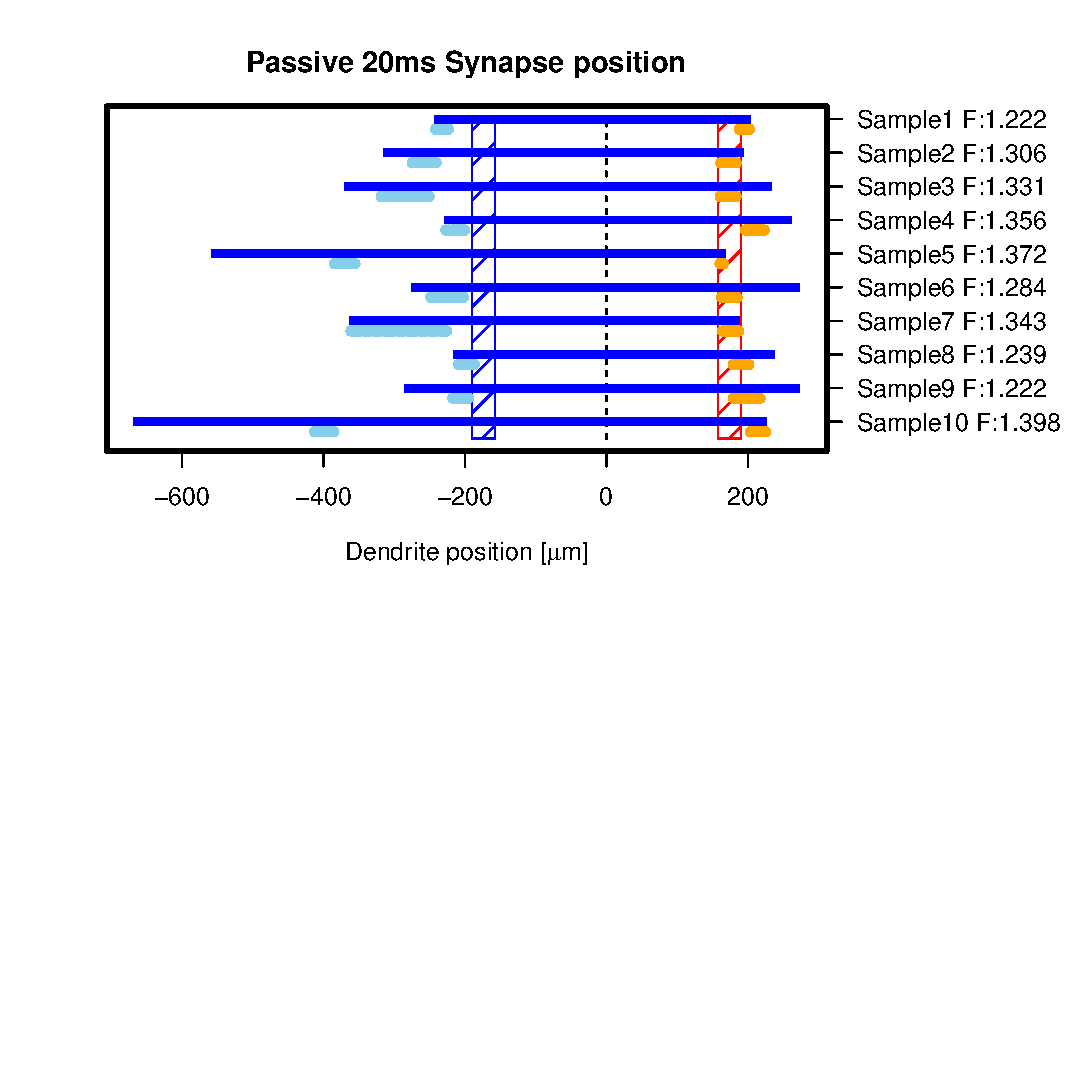
\includegraphics[width=\columnwidth]{./Images_Result/passive_Rerative_75_0_passive_syn_position_dt20.eps}
     %%     \vspace{-5cm}
     %%     \caption{${\Delta}t = 20$}
     %%     \label{passive_syn_dt=20}
     %%   \end{subfigure}

     %%   \hspace*{-2cm}
     %%   \begin{subfigure}{0.62\columnwidth}
     %%     \centering
     %%     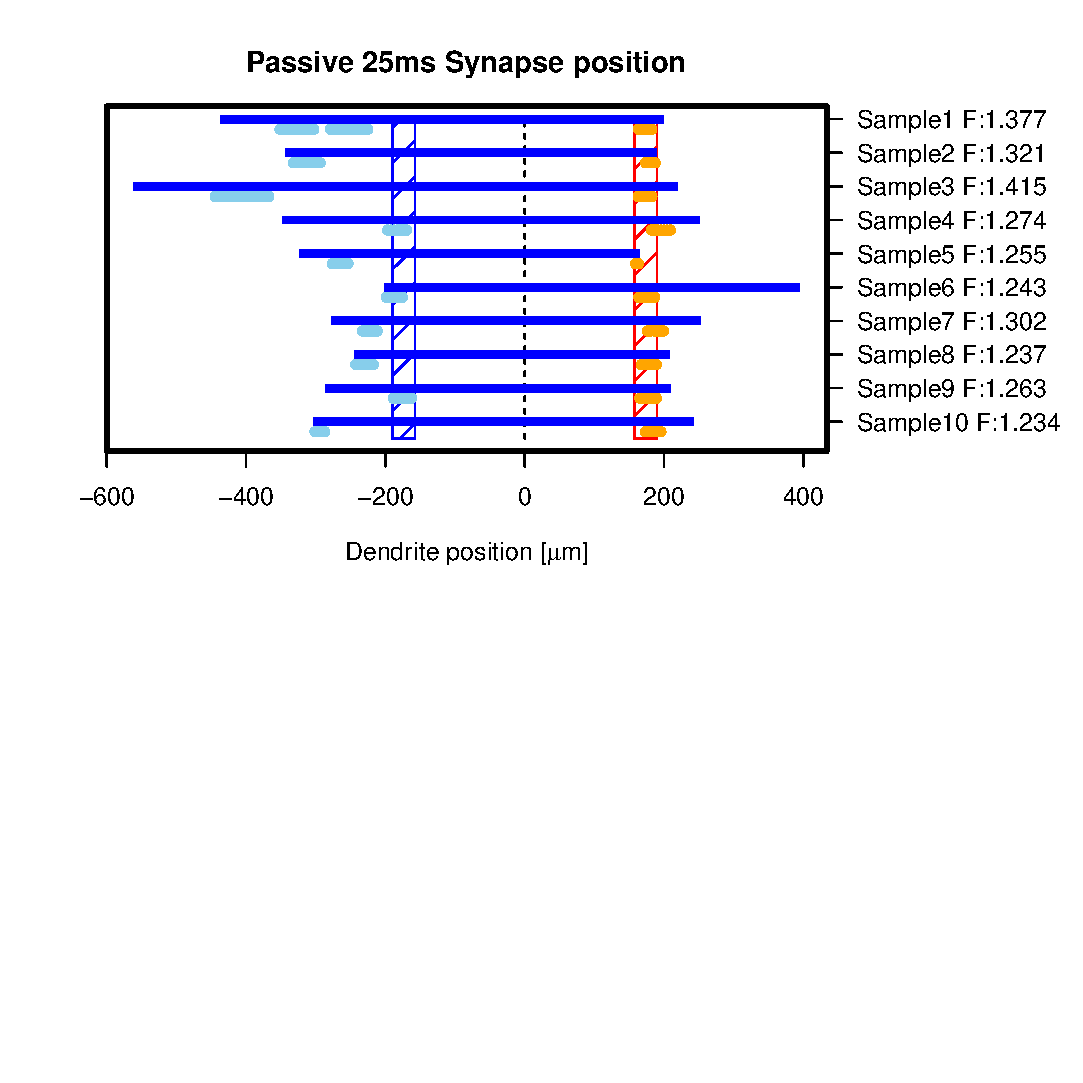
\includegraphics[width=\columnwidth]{./Images_Result/passive_Rerative_75_0_passive_syn_position_dt25.eps}
     %%     \vspace{-5cm}
     %%     \caption{${\Delta}t = 25$}
     %%     \label{passive_syn_dt=25}
     %%   \end{subfigure}
     %%   \begin{subfigure}{0.62\columnwidth}
     %%     \centering
     %%     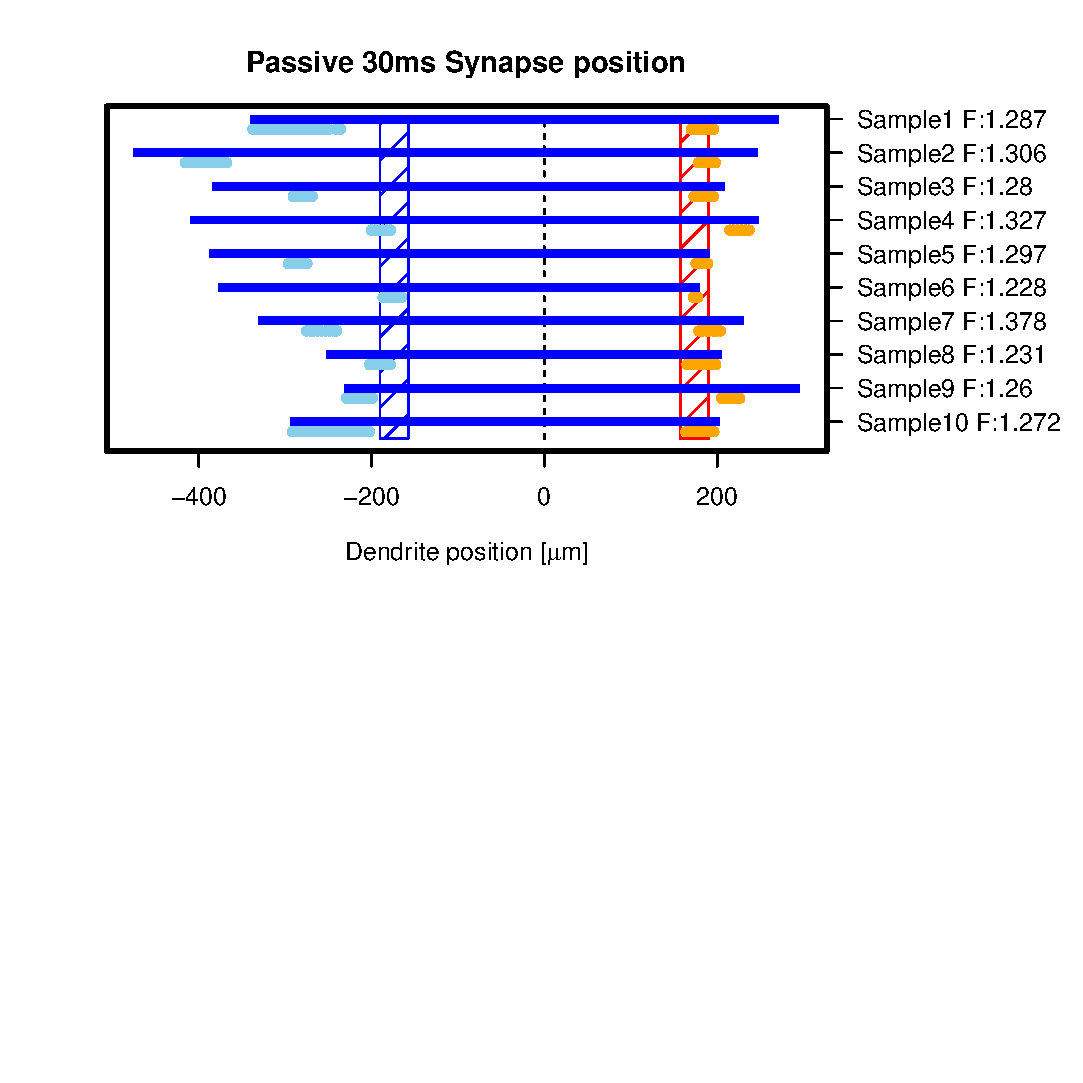
\includegraphics[width=\columnwidth]{./Images_Result/passive_Rerative_75_0_passive_syn_position_dt30.eps}
     %%     \vspace{-5cm}
     %%     \caption{${\Delta}t = 30$}
     %%     \label{passive_syn_dt=30}
     %%   \end{subfigure}

     %%   \vspace{-1cm}
     %%   \begin{subfigure}{\columnwidth}
     %%     \centering
     %%     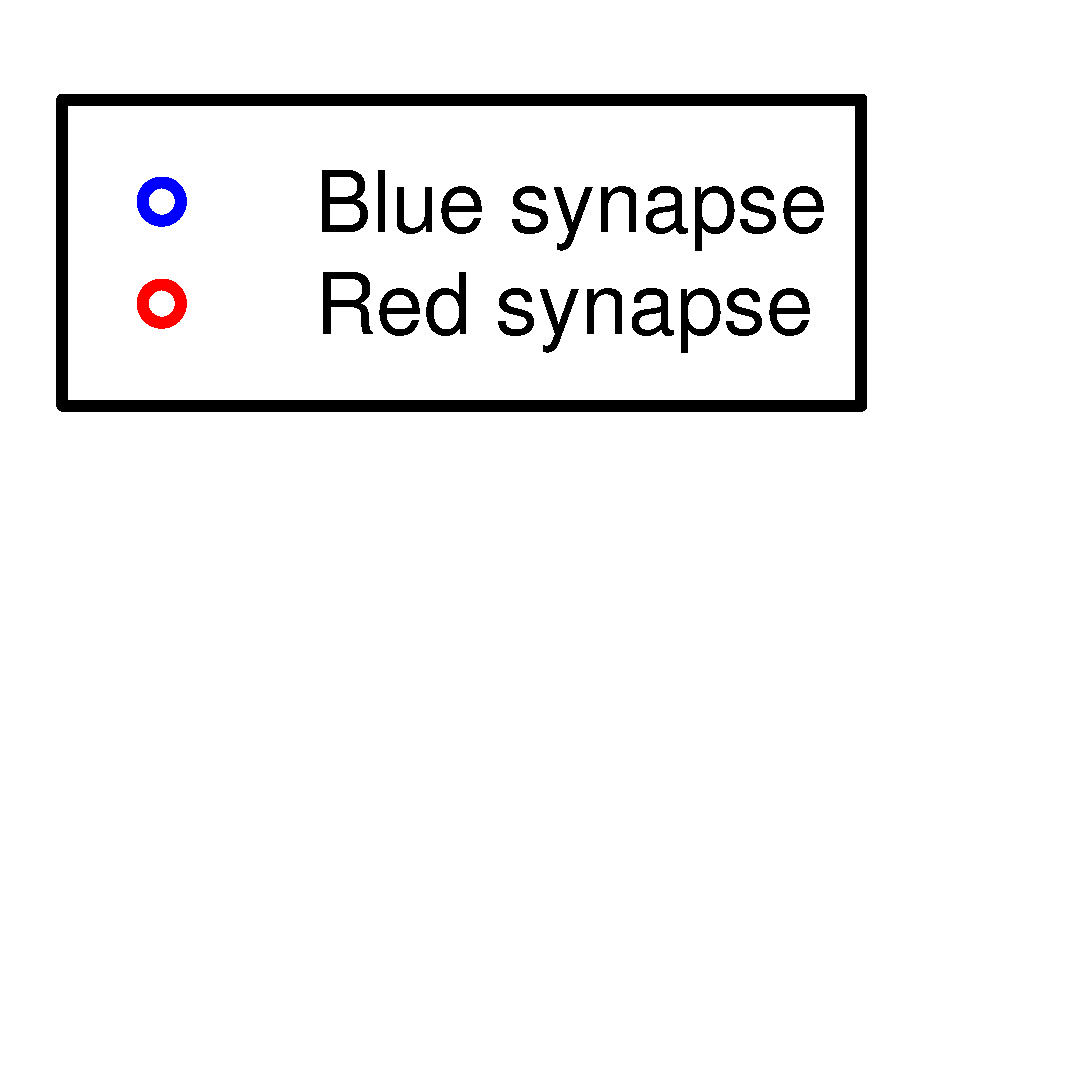
\includegraphics[width=0.3\columnwidth]{./Images_Result/Synapse_legend.eps}
     %%   \end{subfigure}
     %%   \vspace{-3cm}
     %%   \caption{Passive$B$J?@7P:YK&$N%7%J%W%90LCV(B}
     %%   \label{passive_syn}
     %% \end{figure}

     %% $B?^(B\ref{passive_syn}$B$h$j(BUpper Dendrite$B$N7A>u$d%7%J%W%97A@.0LCV$O(B,
     %% ${\Delta}t$$B$K0M$i$:$[$\0lDj$G$"$k$3$H$,$o$+$k(B. $B0lJ}$G(BLower Dendrite$B$N7A>u$O(B
     %% Upper Dendrite$B$h$j$bJQ2=$KIY$s$G$$$k(B.
     %% %$B:G8e$NJ}$,$"$$$^$$(B

